\chapter{Background: GuideaMaps}\label{ch:background-guideamaps}
This chapter provides a description of the first version of the tool. We present the system and explain its limitations to have a good view of the elements we certainly want to improve in our new version. The information is based on the master thesis of Erik Janssens \citep{erikjanssens}, the related publication \citep{detroyerjanssens}, and the last version of the tool.

\section{Goals \& Principles}
GuideaMaps is an iOS-based iPad application based on mind maps. It can be seen as an ideation tool, i.e. a tool that mimics the thinking pattern that people follow when engaged in inventive thinking, e.g. about new products or systems \citep{goldenberg1999ideation}. The name ``GuideaMaps'' is a concatenation of ``Guided'' and ``Ideas'' and each node in the map is called a ``Guidea''. The initial goal of the tool was to provide support for the requirement elicitation process for serious games \citep{erikjanssens}. Later on the tool was extended to also support requirement elicitation for other domains. The only prerequisite is that the requirement elicitation process of the domain is already well known, i.e. it is known which sort of requirements need to be specified for the system in the domain. Therefore, it is called domain-specific requirement elicitation. Example domains are serious games and e-commerce systems.\\

The issues, i.e. requirements, to consider for a particular domain during requirement elicitation are modeled by means of a kind of predefined mind map, called a \textit{Guidea template}. Such a template provides the different issues to consider, explains them, indicates when issues are required and which are optional, provides possible options and alternatives, indicates the impacts of choices, and allows documenting everything.\\

A Guidea template is sub sequentially used to guide the requirement elicitation process of a new system in the given domain. This is done by selecting or deselecting optional issues, selecting possible options, and providing explanations for all decisions made. The result is an actual \textit{GuideaMap}.\\

In the visualization, the main issue, i.e. idea, is positioned in the center, while all sub-ideas are placed around it. Each idea is represented as a node (called Guidea). An example is shown in \autoref{fig:gm1.0-ecommerce}. Mandatory Guideas are linked to their parent by a solid arrow line, while non-mandatory Guideas are linked with a dotted arrow line.\\

The user of a Guidea template cannot change the structure of the map but he can change some aspects of the layout. To allow the user to group related nodes in a visual way, (s)he can change their color. A user can choose to change the color only for the selected node or for the selected node and all its children. Another way to group nodes is by drag and drop, i.e. the user can change the position of the nodes (using drag and drop) until (s)he obtains a configuration that is more suited for the data or the purpose. These principles support the similarity and proximity principle of the Gestalt Psychology Theory \citep{koffka2013principles}

\subsection{Nodes}\label{sec:nodes}
The regular visualization of a node is a rectangle with rounded corners with a title and some content. If there is not enough space for the content in the visual representation of the node, only the beginning of it is visible. The user can read and edit the complete content by double tapping the node. On double tap, a modal is opened and the keyboard is made visible on the iPad to let the user read and/or edit the data. Note that initially, i.e. when starting to create a Guidea map from a template, the content shown (in the visualization) in the nodes is the description for the Guideas given by the creator of the template. Once the user added a motivation or some other type of information for the Guidea, then this will be shown in the visualization.\\

Next to regular Guideas, there is another type of Guideas, i.e. the so-called ``choice nodes''. These nodes allow the user to select a choice from a predefined set of options. For example, the choice node with title ``Gender'' can have three possibilities which can be added to the visualization, i.e. Male, Female or X. Each time an option is selected, a regular node appears with the name of the option as title. In the template, it can be specified how many options can be or must be selected by the user. This restriction is specified by means of ``cardinalities'', i.e. a lower limit and an upper limit for the number of selections. Graphically, these nodes are smaller than the regular ones and only have a title. While it is possible to change the color of regular nodes, choice nodes always have the same color. This difference is made to let them stand out (similarity principle of Gestalt Psychology Theory \citep{koffka2013principles}).\\

Each node (a regular as well as a choice node) can be marked as optional. In that case, it is not mandatory to fill the content of the node or to select a choice (for choice nodes). As already indicated, these nodes can be recognized by the the dotted line that links them to their parent. The user can decide to use the node and add some content to it, or he can deselect the node, i.e. not use it. A deselected node becomes grey and is less opaque than the other nodes.

\subsection{GuideaMaps}
As already explained, the user starts a GuideaMap by selecting a template from a list of available templates. He can create different maps from the same template and at any time, the user can switch between GuideaMaps he created and has been working on. It is also possible to delete an existing GuideaMap.\\

A GuideaMap can be exported by means of email and imported by another user. The email is also providing the content of the GuideaMap in a textual and readable form.

\section{Limitations}\label{sec:guidamaps-limitations}
The first version of the tool works very well but has some limitations we would like to overcome in our version of the system.
\begin{enumerate}
	\item The tool is created for iPad only. Hence, it is not possible to use it on other devices.
	\item The structure of a map, i.e. the nodes and the links, is fixed and defined by a template on which the map is based.
	\item To define a template, you have to use XML. There is no graphical interface to create templates. This can be a hard task for non-ICT schooled people.
	\item The system is not collaborative: people cannot work together and simultaneously on the same GuideaMap.
\end{enumerate}

\begin{figure}[H]
	\centering
	\frame{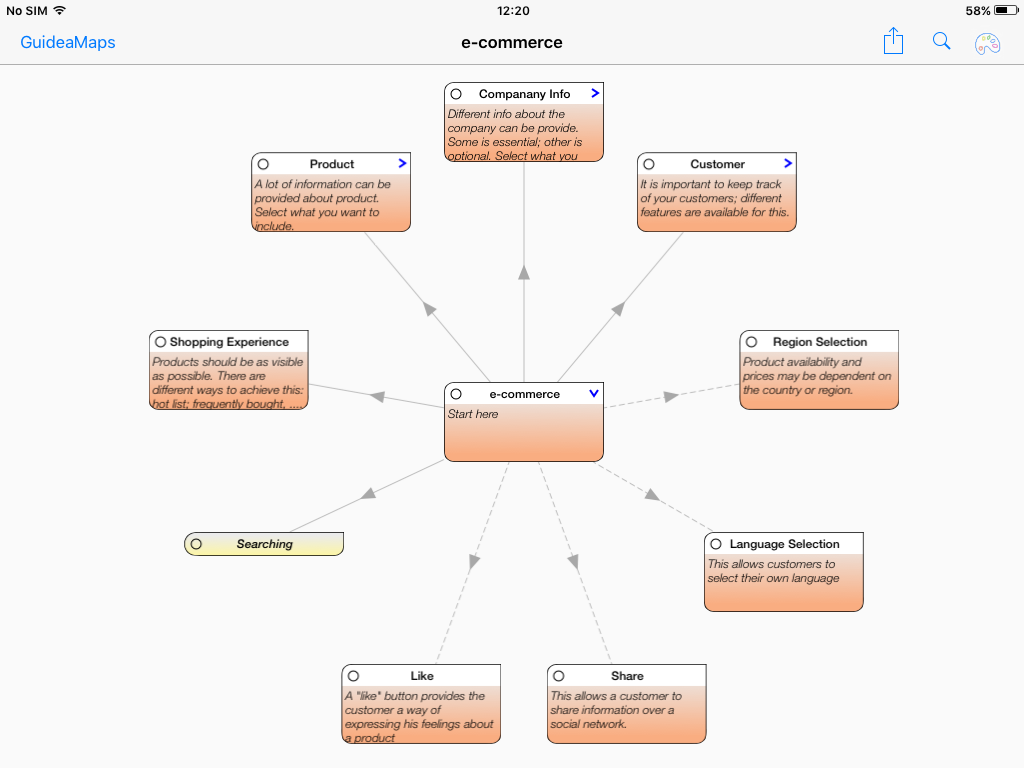
\includegraphics[width=\linewidth]{background/GMversion1ecommerce.png}}
	\caption{E-commerce example created in the original GuideaMaps application.}
	\label{fig:gm1.0-ecommerce}
\end{figure}

